%%%%%%%%%%%%%%%%%%%%%%%%%%%%%%%%%%%%%%%%%%%%%%%%%%%%%%%%%%%%%%%%%%% 
%                                                                 %
%                            CHAPTER                              %
%                                                                 %
%%%%%%%%%%%%%%%%%%%%%%%%%%%%%%%%%%%%%%%%%%%%%%%%%%%%%%%%%%%%%%%%%%% 

\chapter{Literature review}
\label{chap:lit}

\section{State of the art}

	%In this field there is not much research done on implementing direct methods using deep learning and most research is done on the inspection of the resulting workpiece. 
           
		There are a lot of enhancements taking place in the research area of tool wear prediction. The industry 4.0 makes it easier to collect data and process this into usable numbers. 
		A lot of research is performed with this indirectly measured sensor data. For example \cite{Ma2020} uses cutting force as input for a Convolutional Neural Network (CNN) which predicts the tool wear.
		 \cite{Li2013} proposes an in-line set-up which will detect the tool wear and creates an overview of the tool life with three different tool wearing categories namely nose wear, flank wear and crater wear. The wear is displayed for different machining times.  \citeauthor{Li2013} also creates an overview of tests on different materials and different coatings, this gives the reason why it is important to detect tool wear in an early stage to produce high grade products.
		
		 \cite{Cerce2015} provides a way to measure tool-wear with a 3D laser profile sensor. This would be more accurate since more data is available to the algorithms. They divide tool-wear into in two categories: premature tool failure and progressive tool-wear. The premature tool failure "mostly occurs as sudden and unpredictable breakage of the cutting edge" these types of errors won't be detected. The progressive tool-wear on the other hand is easier to predict and measure were the inability of measuring wear profiles in depth is the main disadvantage of direct measuring methods. The results of this paper are really good, they detect the numbers on the crater wear and nose wear of the tool with an accuracy of 1 micrometer. 
		 
		A remarkable study is made by \cite{Pagani2020} who uses the chips cutoff by the tool to predict the tool wear. 
           
           
           Although many researchers choose for indirect measurement methods, some use direct methods like \cite{Ambadekar2020}. They use a microscope to perform off-line tool wear classification in three categories. What they provide is a very similar research as the one done for the set-up verification model which will be implemented later. We will go even further than classification by also predicting the exact flank wear in micrometer. The architecture used by \citeauthor{Ambadekar2020} is Resnet 50 which will also be tested to compare with this study findings. The accuracy achieved is 87\% for the three classes.
           
                 \cite{Schmitt2012} discribes a way of using machine vision to inspect flank wear on cutting tools. The process they use is very labour intensive and should be redone when inspecting a new tool despite this they achieved an accuracy of 7.5 $\mu$m . Their steps are "image acquisition, tool edge detection, highlighting wear region, feature extraction, wear type classification and finally wear measurement." In our paper we will try to make this process a lot simpler by using deep neural networks which will be trained on different tool types. We will need more labelled data to be able to perform such a task which may be expensive to create.
         

            
\section{Information on the process}
\label{sec:lit:reflection}

Our proposal to address this problem of quantizing tool wear consists of using light to reflect on the worn part of the insert into the camera. The image that will be outputted from the camera will then be used to train a neural network that will actually quantize this wear based on the reflection. The characteristics of the carbide inserts will be discussed first along with their reflection. After this the used neural networks will be explained.

\subsection{How does the tool wear?}
	
	The base material of the insert will mostly be Wolfram carbide (WC) for its strength and heat resistance. The same material can also be referred to as Tungsten carbide. This base material is coated with different materials to provide extra strength and durability.
	\cite{Gu1999} Creates an overview of the different wear types with or without coating and the durability under different testing conditions. Figure \ref{fig:alg:insertConstruction} shows how the material is coated and not yet used. 
	The wear of the tool begins with wear on the coating and goes right through the the coating in the base material of the tool. 
	Figure \ref{fig:gen:insertwears} Shows the two types of wear seen on the surface of the inserts. Figure \ref{fig:gen:insertwears}a shows the result of a slow spinning mill where the tool chips off. Figure \ref{fig:gen:insertwears}b shows the wear on an insert which was used under high speeds and where the worn area is flat but not perpendicular to the rake face. This will have to be considered for the light set-up to be able to handle both wear types.
	
	
	\begin{figure}[hbtp]
	\centering
	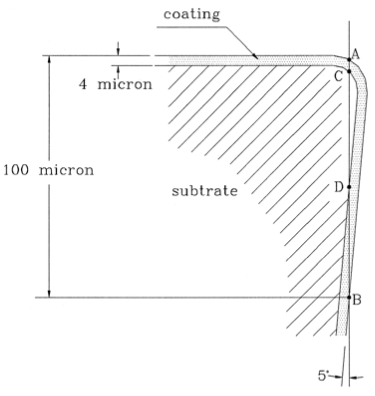
\includegraphics[scale=0.5]{fig/algemeen/plaatjes/Figuren/Insert_construction.png}
	\caption{Construction of the Tool insert with coating. Figure from \citep{Gu1999}}
	\label{fig:alg:insertConstruction}
	\end{figure}
	
	\begin{figure}[hbtp]
	\centering
	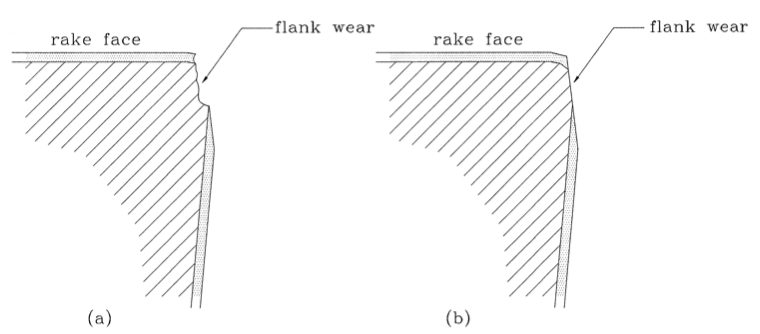
\includegraphics[scale=0.4]{fig/algemeen/plaatjes/Figuren/wear_types.png}
	\caption{Two wear types: (a) Step between substrate and coating. (b) flat wear not perpendicular to the rake face Figure from \citep{Gu1999}}
	\label{fig:gen:insertwears}
	\end{figure}

			
\subsection{Surface of the insert}
\label{sec:lit:surface}
	WC typically has a grain size between 0.5 $\mu$m to 2 $\mu$m which is bonded with cobalt that acts as cement between the WC grains. This declares the name of cemented carbides.
			
			
 The next paper is good to get an overview of the light reflection seen in different types of materials and even multi layered tools where
	\cite{Caicedo2019} researched the reflectance of coating layers on tool inserts. The study suggests that that the best reflection occurs at the highest wavelength. This translates to the visible color red and means that the reflection should be the optimal when the lighting is on the top of the spectrum of the camera. 

%The material is best cut with a laser at wavelengths 1030nm and 515nm. This is proved in: 
%	article: Fundamental investigations of ultrashort pulsed laser ablation on stainless steel and cemented tungsten carbide
%	is the good removal also a good reflector?
		
\subsection{Vision algorithms}
		The problem of tool wear quantisation on carbide inserts is not much researched yet. For this reason there are very little relevant datasets available so the full dataset must be self-created, therefore we will only have a small dataset that consists of a little less than 300 images to work with. Starting from a very small dataset for the creation of a vision set-up, it is necessary to choose a good deep learning network architecture that performs well with little data. This constraints the choice of architectures to the ones with very little training parameters. \cite{Khan2020} extensively describes most available CNN architectures. A few of them are used and repeated underneath for a better understanding of the architectures.
		
		The network will be used to confirm whether a setup is good or not therefore a classification of the images is performed where an image can belong to three classes. 

	%In this section a brief background will be given for the used software and computer vision algorithms. Starting with a listing of different frameworks and continuing with an explanation for the used neural network architectures.
	
	\subsubsection{Frameworks}
	% this section may be deleted
	
		There are many frameworks to perform computer vision tasks and make it easy for the user to get a lot of results in a short amount of time. A list of the used frameworks in this thesis is given below:
		\begin{itemize}
		\item Fast.ai  \citep{fastai} 
		\item Keras \citep{keras} 
		\item PyTorch \citep{pytorch} 
		\end{itemize}
		
		\cite{basnet2019towards} provides an overview of different deep learning frameworks, a short summary of this is given.
		Fast.ai provides a very high level programming experience designed to make deep learning very easy. We found this to be too high level which would affect the customizability of the algorithms.
		Keras is also a high level framework which works with very little programming and is designed for experimenting. 
		PyTorch leaves a little more room for customization. This is the reason PyTorch was used for the most of this thesis. 
		
		
		We will continue with a documentation on the used neural network architectures starting with VGG.
		
	%\subsubsection{Architectures for set-up verification}
	
			\subsubsection{VGG11\_bn}
		VGG is a network architecture found by \cite{Simonyan2015}. It was designed to get better results at the famous Imagenet classification task and does this by using more layers with smaller convolution filters. The original architecture was designed for large scale image classification tasks but will be used for a small dataset in this thesis where a variant of VGG is used with 11 layers instead of the original 19 layered architecture.
		
		The bn stands for batch normalisation which will normalize the output of previous activation layers before passing it on to the next layers. The normalisation will be calculated on every batch instead of the whole dataset.
		
		\subsubsection{Alexnet}
		Alexnet by \cite{Krizhevsky2017} was one of the first to implement deeper structures in the before known CNN architectures. The implementation of deeper network led to overfitting which was countered with including dropout in the fully connected layers. This makes the model more stable even with more layers. At the time Graphics processing units (GPU's) where not as developed as today so the initial architecture consisted of two parallel paths which could run on two separate GPU's. 
		
			\subsubsection{Resnet18}
			First we define what Resnet \citep{He2016} means, after that we dig deeper into the Resnet18 architecture.
			
			Resnet is a deep residual neural network that can reach deeper networks than its predecessors without affecting the complexity of the network. This means that the amount of parameters or the complexity of the training will not increase much when extra layers are added to the model. 
			The depth of the network plays an important role in the performance. 
			
			Figure \ref{fig:vis:resnetBlock} gives an overview of the important building block that lead to the success of Resnet.  Rather than just stacking layers on top of each other, they provide shortcut connections that skip one or more layers. These shortcut connections perform identity mapping where the output of the previous blocks are added to the output of the stacked layers. 
			
			\begin{figure}[hbtp]
			\centering
			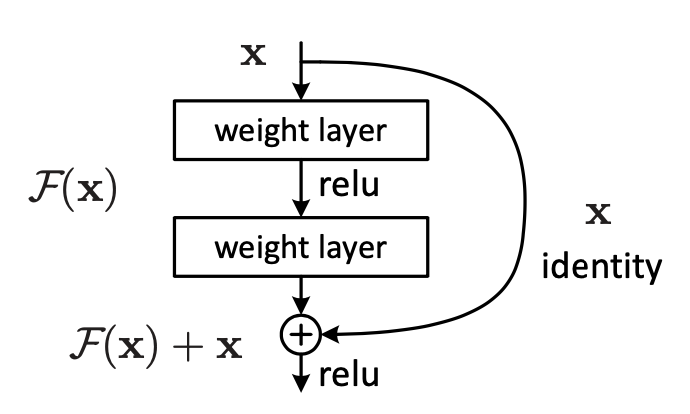
\includegraphics[scale=0.8]{fig/Research/Vision_Algorithm/algorithms/Resnet/resnet_block.png}
			\caption{a building block for Resnet architecture \citep{He2016}.}
			\label{fig:vis:resnetBlock}
			\end{figure}
			
			Figure \ref{fig:vis:resnet18summary} displays a summary of all blocks in the network architecture of Resnet 18. The arrows represent shortcut connections over a few layers. The blocks represent a 3x3 convolution layer where a 3 by 3 grid goes over the previous output and calculates the product with a weight matrix which is updated during training. These calculations provide a new input for the next layer.  The total parameter count for this architecture is 11 million. This seems quite a lot but is actually not much. This will be compared with other network architectures in the next section \ref{sec:lit:va:overview}.
			
			\begin{figure}[hbtp]
			\centering
			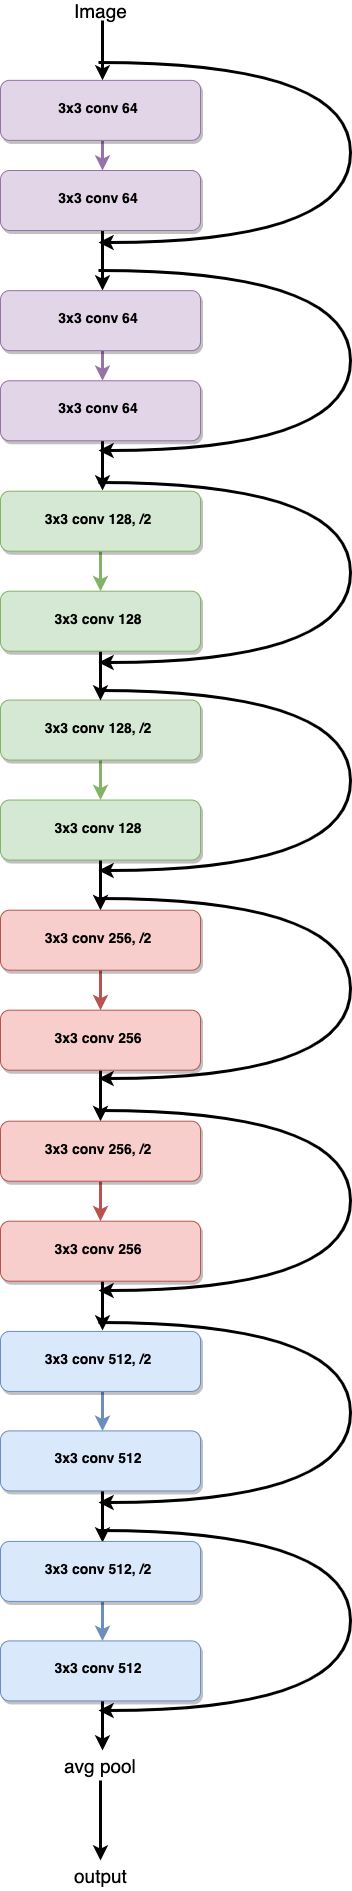
\includegraphics[height=\textwidth, angle=90]{fig/Research/Vision_Algorithm/algorithms/Resnet/Resnet18Diagram.png}
			\caption{Summary of Resnet 18 architecture}
			\label{fig:vis:resnet18summary}
			\end{figure}
			
		\subsubsection{Densenet 121}
		DenseNet \citep{Huang2017} tries to solve the problem of vanishing gradients where information is lost in the back propagation due to too much layers. This is also the problem which ResNet tries to address. ResNet used skip connections to create a bigger information flow to the first layers. DenseNet has a similar aproach where information flow is optimized by connecting every layer to all subsequent layers. This will create better feature propagation through the layers and increase feature reuse. 
		
		A schematic of a dense bloxk is given in Figure \ref{fig:lit:va:denseblock} where the connections are clearly visible. Although we implement DenseNet with 121 layers, it only has 7.9 million parameters to be trained which is an enormous reduction compared with ResNet which has 11.7 million parameters for 18 layers.
		
		\begin{figure}[hbtp]
		\centering
		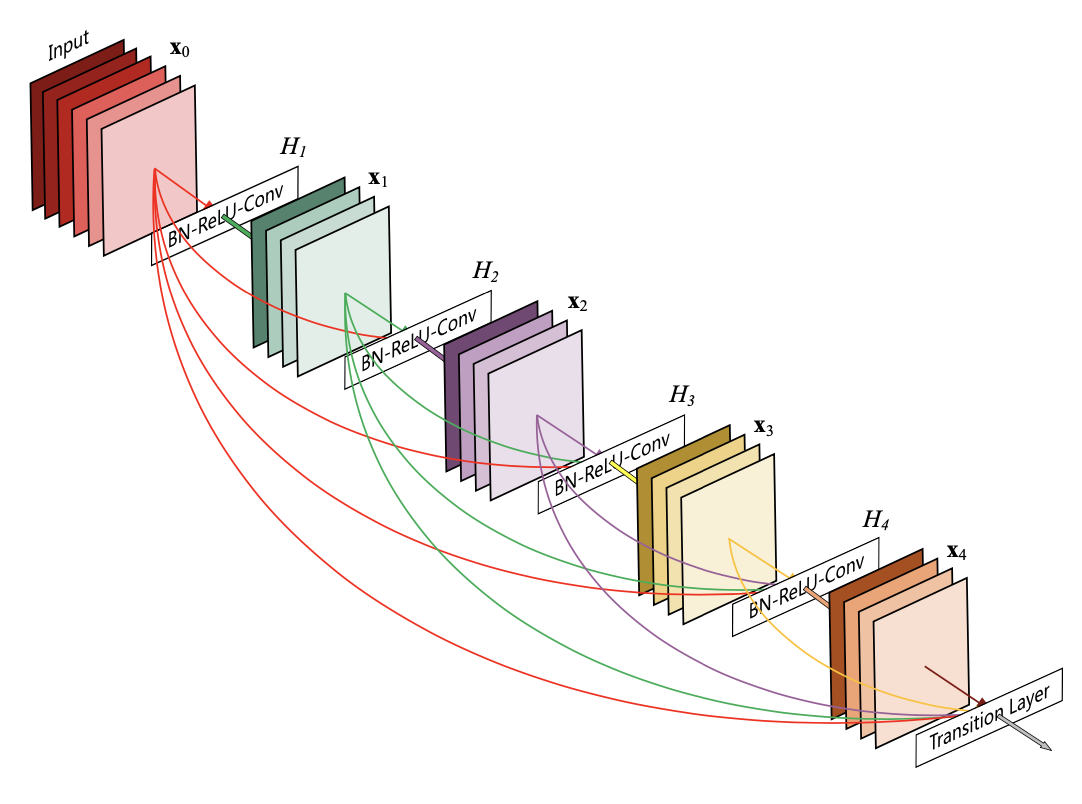
\includegraphics[width=0.49\textwidth]{fig/Research/Vision_Algorithm/algorithms/Densenet/Dense_block.png}
		\caption{Dense block with 5 layers. \citep{Huang2017}}
		\label{fig:lit:va:denseblock}
		\end{figure}
		
		
		\subsubsection{Squeezenet}
		
		If the amount of parameters must be reduced, we can look at implementing Squeezenet which is created by \cite{Iandola2017}. Squeezenet drives the parameter reduction to an extreme where it achieves similar results to AlexNet using 50 times less parameters (1.2 million). The network does this by:
		\begin{enumerate}
		\item Reducing the size of convolution filters from 3x3 to 1x1.
		\item Decreasing the number of input channels by using so-called squeeze layers.
		\item Using delayed downsampling to increase the accuracy without adding much parameters.
		\end{enumerate}
		
		These strategies are incorporated in Fire modules that will be used to form the neural network. 
		
		

	\subsection{Overview of important numbers}
	\label{sec:lit:va:overview}
The amount of parameters and the depth for all architectures are given in table \ref{tab:lit:ov:paramdepth}. These numbers define the complexity of the architecture. Where more layers and more parameters increase the complexity.
	\begin{table}[!ht]
	\centering
	\caption{Parameters and depth in layers for every model accuracy}
\begin{tabular}{c | c c}
			Model name		& parameters (million) 		& depth (layers) \\ \hline
			Resnet 18			&	11.7 			&	18 				\\
			VGG11\_bn			&	123.6 			& 11					\\
			Alexnet				&	61.1 			& 8					\\
			Densenet 121	&	7.9 			& 121				\\
			Squeezenet		&	1.2 			& 10
\end{tabular}
\centering

\label{tab:lit:ov:paramdepth}
\end{table}


\subsection{Other architectures for small datasets}
\label{sec:lit:va:un:other}

%In this section other architectures are explored which received good results on very small image datasets.
%The next data input structure is made:

%	\begin{itemize}
%	\item 20\% train images
%	\item 10\% validation images
%	\item 10\% test images
%	\end{itemize}


%These images will go through different algorithms multiple times and the outputs are verified for every different algorithm.

	Very little datasets are available for this problem so all data used in this thesis will be self created. For this reason there will be very few images to train and test algorithms on. In what follows are some interesting network architectures given for small dataset image classification. These can later be adjusted to perform image regression tasks.
	
	A first architecture is proposed by \cite{Chandrarathne2019}. They compare training a five layered neural network from scratch using transfer learning on the Imagenet dataset. The findings where that transfer learning could increase the testing accuracy by 10\% on small datasets.
	
	\cite{Xu2019} proposes a so called SDD-CNN what stands for small data driven convolution neural network. This was used for the inspection of roller bearings. A preprocessing method called label dilation is used to solve dataset imbalance because there is a big difference in amount of positive and negative examples. This label dilation method generates random samples where the amount of items per class after dilation equals the amount of items in the biggest class before dilation. For the roller bearings there are 300 samples per class. After preprocessing, the images are augmented to extend the dataset in a controlled way using semi-supervised data augmentation. This process is done by cropping the worn area of the bearing rather than center cropping. Then four networks are trained with the received data. These networks are: 
	\begin{enumerate}
	\item Squeezener v1.1
	\item Inception v3
	\item VGG-16 
	\item ResNet-18
	\end{enumerate}

The findings of the research are that inception v3 performed best for this small dataset when used with transfer learning.


			